%Struktur
% -Festlegung von Software-Kriterien
% -Auswahl des Verfahrens
% -Reproduktion des Verfahrens aus der Literatur
% 	-Kantenerkennung
% 	-Segmentierung
%	-Probleme & besondere Erkenntnisse
% -Erweiterung des Verfahrens
%	-Grundlegende Änderungen des Verfahrens
%	-False edge removal
%	-Point marking and cloud filtering
%	-misc.


\chapter{Methodik}
Die Rücksichtnahme des Einsatzzwecks bei der Design und Entwurf des Verfahrens sowie die Entwicklung der Software war erforderlich, um die gewünschte Funktionalitäten gewährleisten zu können. Das Verfahren soll Kanten und Geometrien nicht nur in vollständig generierten Punktwolken erkennen, sondern auch in unvollständige Punktwolken, die iterativ wachsen. Hierbei wird ein Laserliniensensor eine Kante eines Werkstücks oder Objektes entlang geführt und somit sequentiell abgetastet. Deswegen wird die räumliche Struktur des Objektes nicht in einer einzigen Aufnahme abgebildet, sondern durch mehrere kleine Einzelaufnahmen. Der intelligente Schweißroboter, der durch das Fraunhofer Institut für Produktions- und Automatisierungstechnik entwickelt wird, verwendet ein solches Verfahren zum Scannen eines Werkstückes und zur Erkennung Schweißnähte \autocite[39]{savla_intelligente_2022}. Mittels eines Lasersensors wird die Oberfläche des Werkstückes dreidimensional abgebildet. Aktuell wird eine Schweißkegelnaht durch die Erkennung der Schnittlinie zwei Ebenen markiert, die mittels RANSAC-Algorithmen auf die Punktwolke des Werkstückes gefittet werden. Dieses Verfahren zur Erkennung der Schweißnaht bietet allerdings kaum detaillierte Informationen über die Geometrie des Werkstückes an.\autocite[39-52]{savla_intelligente_2022}. Das, in dieser Arbeit entwickelte Verfahren soll das bestehende Verfahren ersetzen und somit seine Limitationen überwinden. %Absatz anpassen. Soll in Einleitung gehen als Stand der Technik.

\begin{figure}[h]
	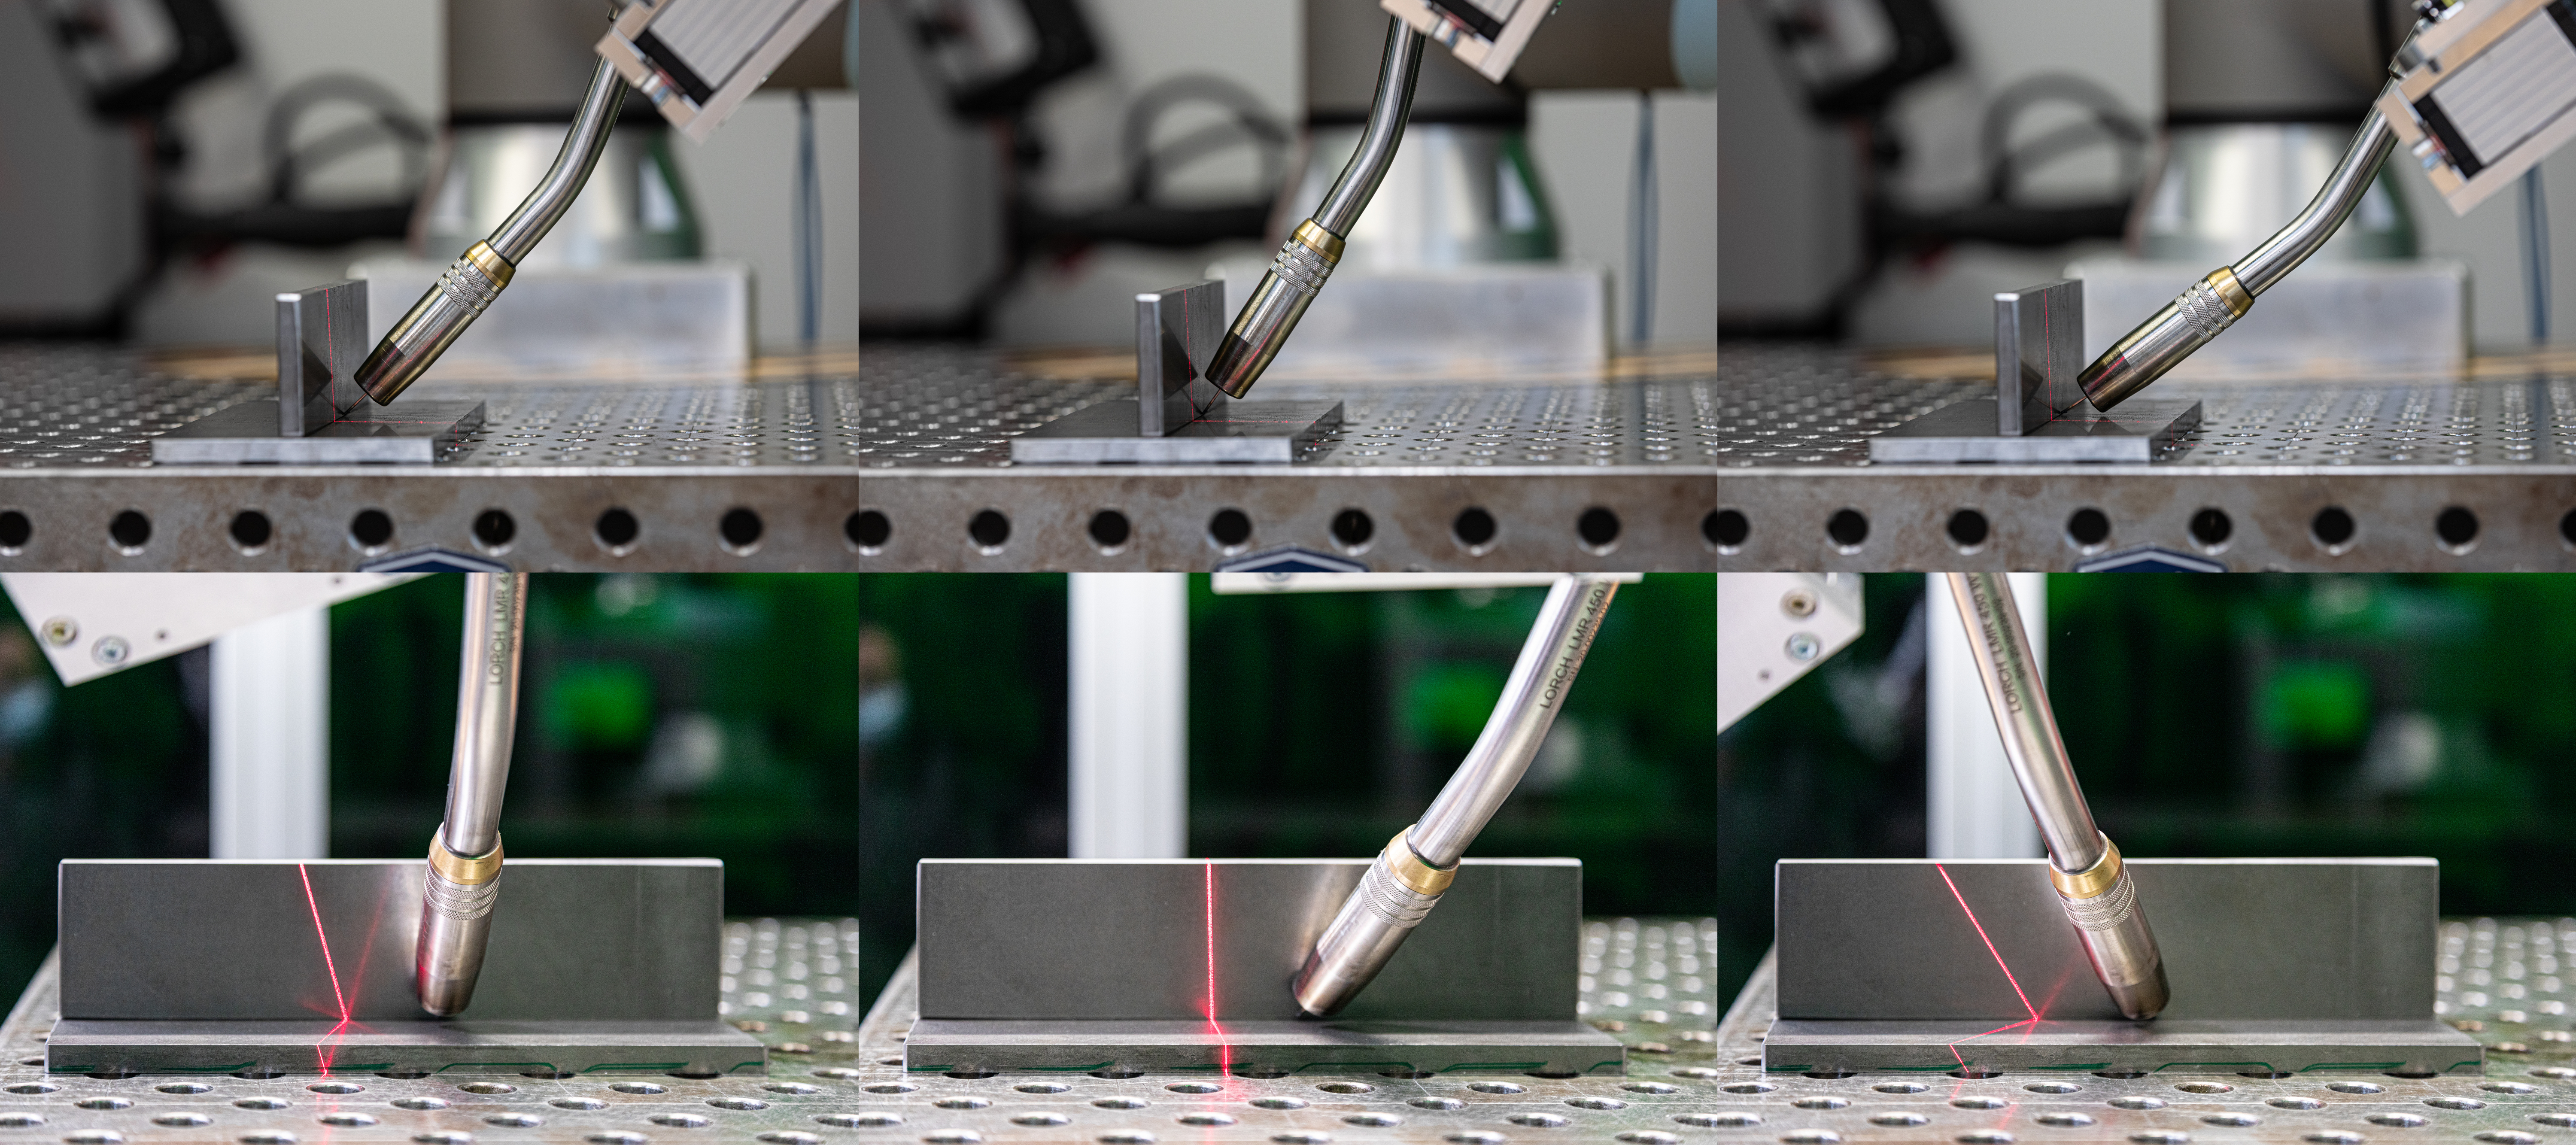
\includegraphics[width = \textwidth]{Abbildungen/collage.jpg}
	\centering
	\caption{Der Laserliniensensor} 
\end{figure}

\section{Vorbereitungen} \label{agpn_reproduction}
\subsection{Software-Voraussetzungen}\label{soft_voraus}
Bei der Auswahl eines geeigneten Verfahrens zur Detektierung Kanten in einer Punktwolke müssen einige Voraussetzungen festgelegt werden. Die Methode soll in der Lage sein, nicht nur Außenkanten zu erkennen, sondern auch Innenkanten beziehungsweise Faltungen. Neben dem originellen Einsatzzweck soll das Verfahren möglichst breit anwendbar sein und eine hohe Modularität aufweisen. Die Funktionen der Kantenerkennung und -Segmentierung soll unabhängig von einander aufrufbar gestaltet werden, um dem Benutzer eine möglichst hohe Flexibilität anzubieten. Die Kantenerkennung soll performant erfolgen und Punktwolken innerhalb eines praktischen Zeitraums verarbeiten. Letztlich soll das Programm in dem bestehenden Programmpaket des Schweißroboters integrierbar sein. Die Hardwarebeschleunigung des Verfahrens mittels eines Grafikprozessors wird ausgeschlossen, da ihrer Verwendung mit dem Echtzeitkernels des Programmpakets zur Konflikte führt. 

\subsection{Auswahl eines Verfahrens}
Eine Literatursuche nach Verfahren zur adaptiven Erkennung von Kanten in wachsenden 3D Punktwolken für den Einsatzzweck ergab nichts. Die meisten Verfahren eigneten sich für die Kantenerkennung nur in vollständigen Punktwolken. Aus diesem Grund wurde die Entscheidung getroffen, ein vorhandenes Verfahren aus der Literatur zu wählen und es für den Einsatzzweck anzupassen. Drei unterschiedlichen Verfahren nach \textcite{bazazian_edc-net_2021}, \textcite{himeur_pcednet_2021} und \textcite{rachmadi_road_2017} zeigten viel versprechende Ergebnisse. Allerdings werden neuronale Netze in dieser Verfahren verwendet, welches zu zwei Problemen geführt hätte. Aufgrund der Funktionsweise neuronaler Netze wäre es schwierig gewesen, diese für den Einsatzzweck ohne eine umständliche Anpassung des neuronalen Netzes anzupassen. Das zweite Hindernis entsteht durch die Einschränkung bei der Verwendung von Grafikprozessoren. Diese Prozessoren hätten die Rechenzeit neuronaler Netze sehr stark verringert und die schnelle Performanz des Verfahrens gewährleistet \autocite[625]{luo_artificial_2005}. Das numerische Verfahren nach \textcite{choi_rgb-d_2013} war auch für den Einsatzzweck ungeeignet, da es für ein Eingangsparameter eine RGB-D Datei erfordert. Somit wäre das Verfahren nur für eine Anwendung auf organisierten, gefärbten Punktwolken eingeschränkt. Es werden zwei weitere Verfahren gefunden, die sich zur Erkennung Kanten in organisierten sowie unorganisierten Punktwolken eignen würden. \textcite{mineo_novel_2019} stellten eine numerische Methoden vor, welche zu einer hohen Genauigkeit Kanten erkennen konnte. Allerdings werden keine Angaben über die Erkennung Innenkanten in dieser Arbeit gemacht. \textcite{ni_edge_2016} schlagen im Gegensatz eine Methode namens AGPN vor, die nicht nur Kanten und Faltungen erkennt, sondern diese zusammen clustert, um geometrisch  voneinander unterschiedlichen Kanten zu trennen. Diese Studie präsentierte ein Verfahren mit einer hohen Genauigkeit sowie eine Möglichkeit, die Kanten sinnvoll zusammen zu gruppieren. Aus diesem Grund wurde dieses Verfahren als Grundlage für das adaptive Verfahren dieser Arbeit gewählt. %Nach aktuellem Kentnisstand ist keine Methode entwickelt worden

\section{Reproduktion des AGPNs}
Bevor das Verfahren für den Einsatzzweck angepasst wird, soll es zuerst zwecks einer Überprüfung unverändert implementiert werden. Es soll sichergestellt werden, dass das Verfahren für die Erkennung Innenkanten und potenzielle Schweißnähte geeignet ist. Da die Autoren das Quellcode ihres Verfahrens nicht öffentlich zugängig gemacht haben, muss das Programm händisch reproduziert werden. Die Reproduktion des Programms erfolgt in zwei Schritten - die Reproduktion des Verfahrens zur Kantenerkennung und dessen zur Kantensegmentierung. Obwohl andere Skriptsprachen wie Python und MATLAB hinsichtlich des Prototypings Vorteile anbieten, wird das Programm in C++ wegen seiner besseren Leistungsfähigkeit implementiert \autocite{svensson_performance_2021}. Viele Funktionalitäten der PCL-Bibliothek \autocite{rusu_3d_2011} werden auch für den Entwurf des Verfahrens verwendet.

\subsection{Verfahren zur Kantenerkennung} \label{edge_detection_reprod}
Während Randelemente in zweidimensionale Bilder eine klare Definition haben, fehlt eine solche Definition für Randelemente und Kanten in 3D-Punktwolken. Es lässt sich erkennen, dass Kanten einer dreidimensionalen Punktwolke aus Randpunkten bestehen. In diesem Verfahren werden die geometrischen Eigenschaften einer Kollektion von Punkten zur Erkennung Randpunkte berücksichtigt. Randpunkte weisen diese besondere geometrische Eigenschaft auf - der Winkelabstand zwischen benachbarten Randpunkte ist im Vergleich zu anderen benachbarten Punkten deutlich größer. Faltungen stellen den Grenzbereich zwischen zwei angrenzenden Ebenen dar, deren Normale in unterschiedlichen Richtungen zeigen. Diese geometrischen Eigenschaften werden zur Erkennung Randpunkte verwendet. \autocite[1-2]{ni_edge_2016}

\begin{figure}[h]
	\includegraphics[scale=0.12]{Abbildungen/ablauf_plan_edge.png}
	\centering
	\caption{Das Programmablaufplan zur Erkennung Randpunkte \autocite{ni_edge_2016}.}
	\label{flow_chart}
\end{figure}

Im folgenden wird die Kantenerkennung detaillierter erläutert, welches ein Teilverfahren des AGPN-Verfahrens ist. Zwecks der Übersichtlichkeit wird dieses Teilverfahren als \textit{FindEdgePoints} referiert. Für einen Punkt \textit{o} wird eine Sammlung von \textit{K\textsubscript{1}} benachbarten Punkten mittels eines kd-trees erstellt. Diese Sammlung wird als eine Nachbarschaft \textit{N\textsubscript{o}} referiert. Danach wird mittels eines RANSAC-Algorithmus eine Ebene \textit{E\textsubscript{N\textsubscript{o}}} auf diese Nachbarschaft gefittet, um Ausreißer herauszufiltern und zwei angrenzenden Flächen innerhalb der Nachbarschaft voneinander zu trennen. Diese Ebene wird als eine RANSAC-Ebene referiert. Danach wird Überprüft, ober der Punkt \textit{o} auf der RANSAC-Ebene liegt. Falls dieser Punkt ein Ausreißer der Ebene \textit{E\textsubscript{N}} ist, kann er keinen Randpunkt sein und das Verfahren wird für einen neuen Punkt wiederholt. Ansonsten werden weiterhin die geometrischen Eigenschaften der Nachbarschaft überprüft. Abbildung \ref{RANSAC-Ebene} visualisiert die Trennung zwischen unterschiedlichen Flächen einer Punktwolke mittels des RANSAC-Verfahrens. 

\begin{figure}[h]
	\includegraphics[width=\textwidth]{Abbildungen/RANSAC-Ebene.png}
	\centering
	\caption{Eine lokale RANSAC-Ebene (rot dargestellt) neben anderen Oberflächen (blau dargestellt). In \textbf{a} sind drei Ebenen zu sehen, wobei in \textbf{b} nur zwei zu sehen sind. \autocite{ni_edge_2016}}
	\label{RANSAC-Ebene}
\end{figure} 

Im Falle, dass der Punkt \textit{o} ein Inlier ist und zu der Ebene \textit{E\textsubscript{N\textsubscript{o}}} gehört, fängt die tatsächliche Überprüfung der geometrischen Eigenschaften der Nachbarschaft \textit{N\textsubscript{o}} an. Um die Ebene von \textit{E\textsubscript{N\textsubscript{o}}} näherungsweise zu schätzen, wird zuerst die Normale \textit{$\vec{n}$} der Ebene geschätzt. Es wird die Ebenengleichung durch das RANSAC-Verfahren näherungsweise geschätzt. Diese Gleichung wird weiterhin optimiert und daraus die Normale \textit{$\vec{n}$} ermittelt. Danach erfolgt die Errechnung des Winkelabstands zwischen den jeweiligen Nachbarpunkte in \textit{N\textsubscript{o}}. Hierfür wird für die Ebene \textit{E\textsubscript{N\textsubscript{o}}} die jeweiligen Eigenvektoren $\vec{u}$ und $\vec{v}$ aus der Normale $\vec{n}$ errechnet. Es gibt ein vorhandenes Verfahren von PCL zur Ausrechnung der Eigenvektoren, allerdings liefert es ungenaue Ergebnisse. Stattdessen werden zur Ermittelung \textit{$\vec{u}$} zwei zufällig gewählte Punkten aus der Inliers verwendet. Es wird dabei sichergestellt, dass keiner der Punkten der Punkt \textit{o} sind. Zur Errechnung des Winkelabstands werden zuerst die Winkel aller Punkte der lokalen Ebene \textit{E\textsubscript{N\textsubscript{o}}} errechnet. Mit dem Punkt \textit{o} als Ursprung wird für jeden Punkt \textit{p\textsubscript{i}}, aus \textit{N\textsubscript{r}} Punkten, der Winkel \textit{$\theta_i$} zu einer Nulllinie errechnet. Danach wird die Differenz zwischen zwei konsekutiver Punktwinkel $\theta_i$ und $\theta_{i+1}$ errechnet, welcher den Winkelabstand \textit{G\textsubscript{$\theta$}} zwischen zwei Punkten - \textit{p\textsubscript{i}} und \textit{p\textsubscript{i+1}} - beträgt. Bei einer Winkelabstand größer als einem bestimmten Schwellenwert $\alpha$ wird der Punkt \textit{o} als ein Randpunkt markiert. Das Referenzwerk verwendet einen Schwellenwert $\alpha$ von $\frac{\pi}{2}$. Abbildung \ref{edge_boundary} zeigt, wie der Winkelabstand zwischen Punkten am Rand der Punktwolke aussieht.

\begin{figure}[h]
	\includegraphics[width=0.5\textwidth]{Abbildungen/angular_gap_boundary}
	\centering
	\caption{Der Winkelabstand \textit{G\textsubscript{$\theta$}} zwischen Punkten am Rand der Punktwolke. \textbf{\(a\)} zeigt ein interner Punkt \textit{o}und ein Nachbarpunkt \textit{p\textsubscript{i}}. Im Vergleich dazu zeigt \textbf{\(b\)} \textit{o} am Rand und den großen Winkelabstand \textit{G\textsubscript{$\theta$}} zwischen Punkte \textit{p\textsubscript{i}} und \textit{p\textsubscript{i + 1}}. \autocite{ni_edge_2016}}
	\label{edge_boundary}
\end{figure}

Auch die Erkennung von Punkten in Innen- und Außenkanten ist durch diese Berechnungen möglich. Wie bereits erwähnt, werden zwei angrenzenden Flächen mittels das RANSAC-Verfahren voneinander getrennt. Falls der Punkt \textit{o} auf der Schnittlinie beider Flächen sowie auf der lokalen RANSAC-Ebene \textit{E\textsubscript{N\textsubscript{o}}} liegt, dann gehört es zum lokalen Rand der Ebene. Falls der Punkt \textit{o} auf der Schnittlinie beider Flächen liegt, aber nicht zu der RANSAC-Ebene gehört, wird er automatisch nicht als ein Randpunkt gemerkt. \textit{E\textsubscript{N\textsubscript{o}}}. Die Abbildung \ref{edge_fold} zeigt, wie der Winkelabstand zwischen Punkten auf einer Schnittlinie zwischen zwei Flächen der Punktwolke aussieht. Die Errechnungen des Winkelabstands erfolgt nach den Gleichungen \ref{first_equation} - \ref{last_equation}.

\begin{figure}[h]
	\includegraphics[width=\textwidth]{Abbildungen/angular_gap_fold}
	\centering
	\caption{Der Winkelabstand zwischen Punkten auf einer Schnittlinie zwei angrenzender Flächen. \textbf{\(a\)} zeigt ein interner Punkt \textit{o} der RANSAC-Ebene. \textbf{\(b\)} zeigt \textit{o} am lokalen Rand der RANSAC-Ebene und den Winkelabstand \textit{G\textsubscript{$\theta$}} zwischen Punkte \textit{p\textsubscript{i}} und \textit{p\textsubscript{i + 1}}. \textbf{\(c\)} zeigt \textit{o} als ein Ausreißer der RANSAC-Ebene. \autocite{ni_edge_2016}}
	\label{edge_fold}
\end{figure}

\begin{equation}
\label{first_equation}
d_i^u = \vec{{op}_i} \cdot \vec{u}
\end{equation}
\begin{equation}
d_i^v = \vec{{op}_i} \cdot \vec{v}
\end{equation}
\begin{equation}
\theta_i = \arctan{\frac{d_i^u}{d_i^v}}
\end{equation}
\begin{equation}
G_\theta = \max(\theta_{i + 1} - \theta_i), i \in \{1, \ldots, N_r - 1\},
\label{last_equation}
\end{equation}


Um die Genauigkeit des Verfahrens zu versichern und die Rechenarbeit des Verfahrens zu verringern, werden gezielt zwei zusätzliche Schritte vor dem Erkennungsverfahren eingeführt. Um die Anzahl der Punkte in der Punktwolke zu verringern, wird ein Voxel-Grid basiertes Downsampling-Verfahren implementiert, um die Punktdichte der Punktwolke künstlich anzupassen und den Abstand zwischen Punkten zu vereinheitlichen. Hierzu dient die PCL-Funktion \textit{UniformSampling} verwendet \autocite{noauthor_point_2023}. Um Ausreißer aus der Punktwolke zu entfernen, wird ein statistisches Verfahren der PCL-Bibliothek namens \textit{StatisticalOutlierRemoval} zur Entfernung von Ausreißer verwendet \autocite{rusu_towards_2008}. Zur Korrekten Ausrechnung des maximalen Winkelabstands einer Nachbarschaft \textit{G\textsubscript{$\theta$}} ist eine aufsteigende Sortierung der Winkel \textit{$\theta_i$} notwendig. Diese Sortierung entspricht eine Sortierung der Punkte \textit{p\textsubscript{i}} nach ihrer aufsteigenden polaren Entfernung von der Nulllinie. Die Abbildung \ref{vector_graph} dient zur Visualisierung der Methode zur Ausrechnung von $\theta_i$. Die Eigenvektoren $\vec{u}$ und $\vec{v}$ bilden das zweidimensionale Koordinatensystem, wobei $\vec{v}$ analog zu einer x-Achse agierte. Die Skalarprodukte \textit{d\textsubscript{i}\textsuperscript{u}} und \textit{d\textsubscript{i}\textsuperscript{v}} repräsentieren die parallelen Anteile des Vektors $\vec{{op}_i}$ der jeweiligen Eigenvektoren $\vec{u}$ und $\vec{v}$. Somit lässt sich der Winkel $\theta_i$ eines Punktes \textit{p\textsubscript{i}} zu der Nulllinie beziehungsweise dem Vektor $\vec{v}$ errechnen. Abbildung \ref{edge_points_table} zeigt die erkannten Kanten einer dreidimensionalen Abbildung eines Tisches.

\begin{figure}[t]
	\includegraphics[scale=0.7]{Abbildungen/vector_graph.png}
	\centering
	\caption{Diese Abbildung stellt die Berechnung des Winkels $\theta_i$ graphisch dar}
	\label{vector_graph}
\end{figure}

\begin{figure}[h]
	\includegraphics[scale=0.37]{Abbildungen/table_edge_overlay.png}
	\centering
	\caption{Die braune Punkte bilden die Ränder bzw. Kanten ab, die in der blauen Punktwolke durch das Verfahren erkannt werden}
	\label{edge_points_table}
\end{figure}

Zusammenfassend wird für jeden Punkt \textit{o} aus der Punktwolke eine RANSAC-Ebene \textit{E\textsubscript{N\textsubscript{o}}} aus einer lokalen Nachbarschaften des Punktes mit \textit{K\textsubscript{1}} Punkten erstellt. Falls \textit{o} auf der Ebene liegt, und der größte Winkelabstand zwischen Punkten der Ebene mit Ursprung \textit{o} größer als $\alpha$ beträgt, wird \textit{o} als ein Randpunkt markiert und gespeichert. Durch die Wiederholung dieser Schritte für alle Punkte können alle Randpunkte und somit aller Kanten der Punktwolke identifiziert werden. Abbildung \ref{flow_chart} stellt den Programmablaufplan für dieses Verfahren dar. Die Probleme bei der Reproduktion dieses Verfahrens werden im Abschnitt \ref{label} besprochen.

\subsection{Verfahren zur Kantensegmentierung} \label{edge_segmentation}
Nachdem die Kanten der Punktwolke erkannt werden, folgt ihrer Segmentierung. Zwecks der Übersichtlichkeit wird das Verfahren zur Kantensegmentierung als \textit{SegmentEdges} referiert. Hierbei werden alle Kanten zusammen gruppiert, die ein geometrisches Merkmal des gescannten Objektes abbilden. Hierfür wird ein Region-Growing Verfahren verwendet. Punkte werden auf Basis zwei Kriterien segmentiert. Das erste Kriterium besagt, dass nur Punkte, die nah aneinander legen, einen Cluster bilden können. Das zweite Kriterium besagt, dass nur Punkte, die in einer ähnlichen Hauptrichtung zeigen, zusammen geclustert werden dürfen. Die Segmentierung erfolgt hauptsächlich in zwei Schritten - die Erstellung und Exaktifizierung von Nachbarschaften sowie die Region-Growing Segmentierung der Kanten. Das Teilverfahren \textit{SegmentEdges} besteht aus zwei weiteren Teilverfahren - \textit{ComputeVectors} und \textit{ApplyRegionGrowing}

Bei \textit{ComputeVectors} handelt es sich um die Berechnung der Richtungsvektoren und die Bestimmung der exakten Nachbarpunkte jedes Randpunktes aller Kanten. Für einen Randpunkt \textit{p} werden \textit{K\textsubscript{2}} Nachbarpunkte aus den, nach \textit{FindEdgePoints} erkannten Randpunkten, gesucht. Diese Sammlung wird als die Nachbarschaft \textit{N\textsubscript{p}} referenziert. Danach wird eine Linie \textit{L\textsubscript{N\textsubscript{p}}} mittels eines RANSAC-Verfahrens auf die Nachbarschaft gefittet, um alle Punkte zu finden, die in der gleichen Hauptrichtung zeigten. Falls der Randpunkt \textit{p} nicht zu den Inliers der RANSAC-Linie gehört, wird die Linie \textit{L\textsubscript{N\textsubscript{p}}} iterativ so lange angepasst, bis \textit{p} zu den Inliers von \textit{L\textsubscript{N\textsubscript{p}}} gehört. Danach werden alle Inliers der Linie \textit{L\textsubscript{N\textsubscript{p}}} als die exakten Nachbarpunkte des Punktes \textit{p} gespeichert. Der, aus \textit{L\textsubscript{N\textsubscript{p}}} ermittelte Richtungsvektor wird dem Punkt \textit{p} zugeordnet. Dieses Verfahren wird für jeden Randpunkt wiederholt.

Bei \textit{ApplyRegionGrowing} handelt es sich um die Implementierung des Region-Growing-Algorithmus. Hierfür wird das bestehende Region-Growing Verfahren der PCL-Bibliothek adaptiert \autocite{rusu_3d_2011}. Zuerst werden alle Punkte mit dem Label \textit{-1} markiert, um diese als \textit{unsegmentiert} zu kennzeichnen. Das Referenzwerk deutet auf die Irreversibilität des Verfahrens hin, weswegen die Auswahl eines guten Startpunktes sehr wichtig ist. Randpunkte mit einer hohen Anzahl von exakten Nachbarn können mit einer höheren Wahrscheinlichkeit eine Kante oder ein geometrisches Merkmal abbilden. Deswegen sollen alle Randpunkte nach einer absteigenden Anzahl von Nachbarpunkte sortiert werden, sodass die Auswahl eines guten Startpunktes gewährleistet wird. Für den Zuwachs eines Segments \textit{C} wird ein initialer Seedpunkt \textit{s\textsubscript{i}} gewählt, welcher im Falle des ersten Segments der Startpunkt ist. Für jeden unmarkierten (durch \textit{-1} gekennzeichnet) exakten Nachbarpunkt \textit{n\textsubscript{s}} von \textit{s} wird geprüft, ob dessen Hauptrichtungsvektor mit dem des Seedpunktes näherungsweise übereinstimmt. Dies erfolgt durch die Berechnung des Winkelabstands zwischen beiden Hauptrichtungsvektoren, der nicht einen Schwellwert, den sogenannten Glättungsfaktor $\phi$ nicht übersteigen darf. Falls der Richtungsvektor des Nachbarpunktes mit dem des Seedpunktes übereinstimmt, wird es dem Segment \textit{C} hinzugefügt und mit dem Index des Segments markiert. Danach wird \textit{n\textsubscript{s}} zu einer Sammlung neuer Seedpunkte \textit{s\textsubscript{c}} hinzugefügt, die für den weiteren Zuwachs des Segments \textit{C} verwendet werden. Nachdem alle exakte Nachbarpunkte von \textit{s\textsubscript{i}} markiert werden, wird dieser Schritt für alle neue \textit{s\textsubscript{c}} wiederholt, bis die Richtungsvektoren keiner Punkte mit dem von \textit{s\textsubscript{i}} übereinstimmen. Diese Schleife soll zwecks der Wiederverwendbarkeit auf eine separate Methode namens \textit{GrowSegment} verlagert werden. Danach wird ein neuer unmarkierter initialer Seedpunkt \textit{s\textsubscript{i}} gewählt und das ganze Verfahren wiederholt. Im Anhang \ref{label} wird das Verfahren ausführlicher als Pseudocode angegeben. Die Abbildung \ref{segments_table} zeigt alle Segmente in unterschiedlichen Farben an, die durch Region-Growing Verfahren aus den Kanten des Tisches erkannt werden.

\begin{figure}[h]
	\includegraphics[width=\textwidth]{Abbildungen/table_segments.png}
	\centering
	\caption{Diese Abbildung zeigt die, durch das Verfahren erkannte  Segmente des Tisches aus Abbildung \ref{edge_points_table}.}
	\label{segments_table}
\end{figure}

\subsection{Erkenntnisse zu der Reproduktion des AGPNs}
Das \textit{FindEdgePoints} Verfahren soll möglichst schnell erfolgen, um für den Einsatz in der Schweißrobotik geeignet zu sein. Durch die Implementierung des Programmes in C++ erfolgt die Erkennung von Kanten schneller im Vergleich zu anderen Sprachen wie Python oder MATLAB. Allerdings wird die Leistungsfähigkeit moderner Rechner und CPUs durch das Programm nicht völlig ausgeschöpft. Moderne Mehrkernprozessoren bieten die Funktionalität an, Aufgaben parallel auszuführen. Isolierte Rechenaufgaben, die möglichst homogen bleiben und wiederholt werden, lassen sich sehr gut parallelisieren. Das \textit{FindEdgePoints} Verfahren verwendet eine Schleife zur Bestimmung Randpunkte aus allen Punkt der Punktwolke, weswegen es sich zur Parallelisierung eignet. Die Programmierschnittstelle OpenMP bietet über Compiler-Befehle die Möglichkeit an, Prozesse in C, C++ und Fortran zu parallelisieren. Das Schleifenelement des Verfahrens kann mittels OpenMP parallelisiert werden, da die Festlegung eines Punktes zum Randpunkt keinen Einfluss auf die Erkennung anderer Randpunkte hat, und somit eine isolierte Aufgabe darstellt. Es soll auch sichergestellt werden, dass eine Variable in einer Speicheradresse nicht gleichzeitig durch zwei oder mehrere parallelen Instanzen der Schleife überschrieben wird. Auch Datenstrukturen sollen sorgfältig nach ihrer Eignung zur Parallelisierung gewählt werden, um Speicherlecks zu vermeiden. Auch die Berechnung des Winkels $\theta_i$ für jeden Punkt der RANSAC-Ebene \textit{E\textsubscript{N}} könnte parallelisiert werden. Eine solche Parallelisierung bringt eine deutliche Leistungssteigerung mit. 


\begin{figure}[h]
	\centering
	\begin{subfigure}[h]{0.49\textwidth}
		\includegraphics[width=\textwidth]{Abbildungen/blech_edges.png}
		\centering
		\caption{Randpunkte mit PCL 1.12}
		\label{fig: blech_edges}
	\end{subfigure}
	\hfill
	\begin{subfigure}[h]{0.49\textwidth}
		\includegraphics[width=\textwidth]{Abbildungen/blech_bad_edges.png}
		\centering
		\caption{Randpunkte mit PCL 1.10}
		\label{fig: bad_edges}
	\end{subfigure}
	\caption{Randpunkte, die durch beider Versionen von PCL erkannt werden}
	\label{fig: pcl_version_comparision}
\end{figure}

Die zweite Erkenntnis bei der Reproduktion des AGPN Verfahrens ist für die Implementierung auf einem Linux-basierten System relevant. Die Kantenerkennung erfolgt auf die neuere Version des Betriebssystems - Ubuntu Jammy Jellyfish (Version 22.04) - reibungslos und liefert sehr gute Ergebnisse. Die Wiederholung des Programms auf eine ältere Generation des Betriebssystems - Ubuntu Focal Fossa (Version 20.04) - liefert im Gegensatz schlechtere Ergebnisse. Ein Fehler seitens der Hardware kann ausgeschlossen werden, indem der gleiche Rechner mit konstanten Spezifikationen für beide Betriebssysteme verwendet wird. Auch der Einfluss fremder Softwarepakete auf dem Programm kann ausgeschlossen werden, indem das Programm an Betriebssysteme nur mit den notwendigen Softwareabhängigkeiten ausführt wird. Eine genauere Untersuchung liefert den Hinweis, dass die Standardversion der PCL-Bibliothek für beide Betriebssysteme unterschiedlich ist. Die PCL-Bibliotheksversion 1.10 wird Standardweise mit Ubuntu Focal Fossa geliefert, wobei die Version 1.12 Standardweise mit Ubuntu Jammy Jellyfish geliefert wird. Das Downsampling-Verfahren aus der Bibliotheksversion 1.10 kann sehr dichte Punktwolken nicht korrekt verarbeiten. Dieses Fehler wurde allerdings in der neueren Version der Bibliothek behoben. Deswegen wird es empfohlen, entweder die Ubuntu Version 22.04 zu verwenden oder die Standardversion der PCL-Bibliothek zu entfernen und stattdessen die Version 1.12 zu verwenden. Abbildung \ref{fig: pcl_version_comparision} zeigt die Randpunke und im weiteren Sinne die Kanten, die nach dem fehlerhaften Downsampling erkannt werden.

%Nachdem die Funktionsweise des AGPNs getestet wurde, erfolgte die Erweiterung des Verfahrens, um die Kantenerkennung und Segmentierung für wachsenden Punktwolken zu ermöglichen.

\section{Erweiterung des AGPNs - das IEFD}
\subsection{Erstellung der Testumgebung}
Um das Verhalten einer wachsenden Punktwolke zu simulieren und das modifizierte Verfahren zu testen wird eine Testumgebung mittels das Softwarepaket ROS aufgebaut. Die Entscheidung für dieses Softwarepaket stammt aus der Tat, dass es bereits zur Kopplung unterschiedlicher Komponenten des Schweißroboters verwendet wird \autocite[39]{savla_intelligente_2022}. In der Umgebung wird ein ROS-Publisher zur Veröffentlichung der Punkten aus der Punktwolke sowie ein ROS-Subscriber zur Verarbeitung dieser Punkten entworfen. Das ROS-Publisher liest eine Punktwolke-Datei ein, die durch einen Lasersensor aufgenommen wird, und bereitet sie zur Veröffentlichung vor. Die gesamte Punktwolke wird so aufgeteilt, dass es die einzelnen Aufnahmen eines Lasersensors entspricht. Diese aufgeteilten Punkten der gesamten Punktwolke werden als Scan-Linien bezeichnet, da sie eine streifenartige Aufnahme ähneln. Um den Einfluss der Robotergeschwindigkeit zu modellieren, werden diese Scan-Linien mit einer Frequenz von 10 Hz publiziert. Daneben wird der Richtungsvektor des Sensors auch ermittelt und zur Veröffentlichung bereitgestellt. Dieser Vektor gibt an, in welcher Richtung der Sensor verläuft und wird bei der Kantensegmentierung verwendet. Das ROS-Subscriber übernimmt die Aufgabe der Kantenerkennung und -Segmentierung. Die freigegeben Daten aus dem ROS-Publisher werden hier empfangen. Eine Anzahl \textit{n} der empfangenen Scan-Linien werden gesammelt und in einer Punktwolke zusammengefasst, bevor die Kantenerkennung und Segmentierung darauf erfolgt. Danach werden die nächsten \textit{n} Scan-Linien gesammelt und verarbeitet. Diese Anzahl \textit{n} wird dynamisch auf Basis des Abstands zwischen Punkten ermittelt. Die \textit{n} Scan-Linien und deren Verarbeitung wird als eine Iteration referenziert. Innerhalb des ROS-Subscribers werden die Methoden des reproduzierten AGPNs aufgerufen, um Kanten aus der Sammlung von Scan-Linien zu erkennen. Danach werden die Kanten mittels des Region-Growing Verfahrens segmentiert. Diese Kanten und Segmente werden intern gespeichert und mit neuen Kanten nach jeder Iteration erweitert. Zwecks der Datenvollständigkeit werden die letzten \textit{k} Scan-Linien einer Iteration aufgespeichert und am Anfang der nächsten Iteration angehängt. Visualisiert wird das in der Abbildung \ref{fig: point_overlap}. Der Hintergrund dazu wird detaillierter in Abschnitt \ref{false_edges} erläutert.

\begin{figure}[t]
	\includegraphics[scale=0.75]{Abbildungen/points_overlap.png}
	\centering
	\caption{Diese Abbildung visualisiert die Überlappung aufeinanderfolgender Iterationen von Punkten. Zwecks der Übersichtlichkeit werden nur Randpunkte abgebildet. Die vier Farben kennzeichnen Kanten aus jeweils unterschiedlichen Iterationen. Die roten Strichlinien weisen auf dem Ende einer Iteration hin.}
	\label{fig: point_overlap}
\end{figure}

\subsection{Anpassung der Erkennungs und Segmentierung-Verfahren}
Im folgenden werden die Änderungen zu dem AGPN-Verfahren aus Abschnitt \ref{agpn_reproduction} detailliert erläutert. Das angepasste Verfahren wird weiterhin als das \textit{IEFD}-Verfahren \textit{\(\text{Iterative Edge and Feature Detection}\)}refereiert. Die zwei Teile des AGPNs - Erkennung und Segmentierung - werden zwecks der Anpassung als zwei getrennte Funktionen betrachtet. Die Kantenerkennung benötigte keine Änderungen, da der geometrischer Zusammenhang zwischen den Sammlungen von Scan-Linien unterschiedlicher Iterationen keine wichtige Rolle für diese Funktion spielte. Deswegen wird die Funktion \textit{FindEdgePoints} ohne Änderungen für den Einsatz bei wachsenden Punktwolken verwendet. Im Gegensatz dazu, muss das \textit{SegmentEdges} Verfahren angepasst werden.

Bei \textit{SegmentEdges} spielt der geometrischer Zusammenhang zwischen Kanten der unterschiedlichen Iterationen eine wichtige Rolle. Um vorhandene Segmente mit neuen Kanten zu erweitern, sind die relativen Positionen aller Kanten zu einander wichtig. Methoden zur Hinzufügung neuer Randpunkte und im weiteren Sinne, Kanten, zu den Segmenten werden bereitgestellt. \textit{ComputeVectors} kann ohne große Anpassung implementiert werden. Es soll sichergestellt werden, dass nur die neu hinzugefügten Punkte bei diesem Verfahren berücksichtigt werden. Für das \textit{ApplyRegionGrowing} Verfahren muss zuerst die Anzahl und Indizes der bereits erkannten Segmente für die nächsten Iterationen zur Verfügung gestellt werden. Es soll bei jeder Iteration geprüft werden, ob neue Randpunkte zu bereits vorhandenen Segmenten hinzugefügt werden könnten. Zur Erweiterung bestehender Segmente oder Cluster wurden grundsätzlich zwei Verfahren entwickelt. Beide Verfahren werden zwecks der Übersichtlichkeit auf eine separate Methode \textit{ExtendSegment} verlagert.

Bei dem ersten Verfahren werden neue Randpunkte darauf geprüft, ob sie vorhandene Segmente erweitern könnten. Während der Segmentierung werden die exakten Nachbarpunkte eines Punktes \textit{p} durchgesucht, um deren Segment zu finden. Falls einer der Nachbarpunkte bereits zu einem Segment \textit{C} gehört, werden die Richtungsvektoren des Segments sowie des Punktes \textit{p} verglichen. Der Richtungsvektor des Segments wird aus der Summe der Richtungsvektoren aller Punkte des Segments ermittelt. Falls die beiden Richtungsvektoren eine hohe Kollinearität aufweisen, wird es versucht, den Segment \textit{C} mit diesem Punkt zu erweitern. Hierfür wird die Methode \textit{GrowSegment} aus dem \textit{ApplyRegionGrowing}-Verfahren wiederverwendet. Der neue Randpunkt \textit{p} wird als initialer Seedpunkt \textit{s\textsubscript{i}} innerhalb dieser Methode verwendet. Die Richtungsvektoren der unmarkierten exakten Nachbarpunkte von \textit{p} werden mit dem Richtungsvektor des Segments verglichen. Die Nachbarpunkte mit übereinstimmenden Richtungsvektoren werden zu dem Segment \textit{C} hinzugefügt und als neuer Seedpunkt \textit{s\textsubscript{C}} für die Erweiterung von \textit{C} verwendet. Falls der neue Randpunkt \textit{p} zu keinem vorhandenen Segment passt, wird mit ein neues Segment mittels des \textit{GrowSegment}-Verfahrens erstellt.

\begin{figure}[b!]
	\includegraphics[width = 0.95\textwidth]{Abbildungen/blech_segments_bad.png}
	\centering
	\caption{Die falsch segmentierten horizontalen Kanten}
	\label{fig: bad_segments}
\end{figure}

Die erste Methode lieferte unzureichende Ergebnisse, da neuer Randpunkte einer neuen Iteration immer zu einem neuen Segment zugewiesen wurden, obwohl sie offensichtlich zur Erweiterung älterer Segmente geeignet waren. Dieses wird in Abbildung \ref{fig: bad_segments} visualisiert. Deswegen wird eine zweite Variante präsentiert, die \textit{SegmentEdges}-Verfahren nochmal anpasst. In der zweiten Variante darf das \textit{FindEdgePoints}-Verfahren auch unverändert bleiben. Die Verfahren \textit{ComputeVectors} sowie \textit{ApplyRegionGrowing} werden in dieser Variante angepasst. Die \textit{k} wiederholten Punkte und die, daraus erkannten Randpunkte aus jeder Iteration sind für diese zweite Variante wichtig. Die eindeutigen Indizes der wiederholten Randpunkten werden in der Methode \textit{ComputeVectors} verwendet, um deren exakten Nachbarn sowie Richtungsvektoren erneut zu berechnen. Somit werden die neuen Randpunkte aus der neuen Iteration bei der Berechnung der exakten Nachbarn und des Richtungsvektors miteinbezogen. Dadurch werden die örtlichen Relationen zwischen den Randpunkten an den Grenzbereichen zwischen zwei Iterationen etabliert. Diese geometrischen Beziehungen werden später für die Segmentierung relevant.

Das \textit{ApplyRegionGrowing} Verfahren wendet auch die wiederholten Randpunkte aus der vorherigen Iteration an, um vorhandene Segmente zu erweitern. Die Überprüfung jeder einzelnen neuen Randpunkt auf seine Eignung zur Erweiterung eines vorhandenen Segments aus der ersten Variation wird zugunsten eines besseren und effizienteren Verfahrens ersetzt. Bei diesem Verfahren werden Kennzeichnungen aller bereits markierten Punkte in einer neuen Datenstrukturkopie aufgespeichert. Die Kennzeichnung der wiederholten Randpunkte wird auf \textit{-1} zurückgesetzt. Auch die Kennzeichnungen aller exakten Nachbarpunkte dieser Randpunkte werden auf \textit{-1} zurückgesetzt. Danach wird jeder wiederholter Randpunkte \textit{p\textsubscript{r}} wiederverwendet, um sein älteres Segment zu erweitern. Hierbei wird die \textit{GrowSegment} Methode wiederverwendet. Nach der Neusegmentierung der wiederholten Randpunkte werden die Punkte aus der vorigen Iteration darauf überprüft, ob sie unmarkiert (mit \textit{-1} markiert) geblieben sind. In diesem Fall wird die originelle Kennzeichnung dieser Punkte aus der Datenstrukturkopie aufgerufen und den Punkten wieder zugewiesen. Danach werden die übrigen unmarkierten Randpunkte aus der neuen Iteration verwendet, um neue Segmente zu erzeugen. Diese Variante der Methode \textit{ExtendSegment} liefert im Gegensatz zu der ersten Variante deutlich bessere Ergebnisse.

Es soll bemerkt werden, dass aufgrund des IEFD-Verfahrens Punkte zwischen zwei Iterationen fälschlicherweise als Kanten erkannt werden. Diese haben die Genauigkeit der \textit{SegmentEdges}-Verfahren deutlich beeinträchtigt. Im folgenden werden Methoden zur Erhebung dieser falschen Kanten ertönt.

\subsection{Anomalie der falschen Kanten} \label{false_edges}
Aufgrund der Funktionsweise des \textit{FindEdgePoints} Verfahrens werden fälschlicherweise Punkte zwischen zwei Iterationen als Kanten erkannt, obwohl sie im Kontext des Gesamtbildes keine Kanten seien sollten. Je nach Iteration gibt es bis zu zwei Reihen von Punkten, die irrigerweise als Kanten markiert werden. Die erste sowie die letzte Iterationen haben am Ende beziehungsweise am Anfang Scan-Linien, die als Kanten markiert werden. Der Grund hierfür liegt daran, dass die Kantenerkennung nur im Umfang einer Iteration erfolgt und es keine Auskünfte kommende Punkte vorhanden sind. Diese falschen Kanten sind in Abbildung \ref{fig: false_edges} zu sehen. Diese falsch-markierten Kanten haben auf das iterative \textit{SegmentEdges} Verfahren schlechte Auswirkungen und verhindern die Erweiterung bestehender Segmente. Um diese Kanten und im weiteren Sinne, Randpunkte, zu entfernen werden zwei Methoden vorgeschlagen.

\begin{figure}[h]
	\includegraphics[width = 1.0\textwidth]{Abbildungen/false_edges.png}
	\centering
	\caption{Diese Abbildung zeigt die Kanten, die durch das adaptierte Verfahren erkannt werden. Die regelmäßigen durchquerenden Linien in der Mitte, die in Abbildung \ref{fig: blech_edges} abwesend sind, werden fälschlicherweise als Kanten markiert. }
	\label{fig: false_edges}
\end{figure}

\subsubsection{Erste Methode zur Entfernung falscher Kanten}
Bei der ersten Methode wird es versucht, mittels eines Rahmens - ein sogenanntes Bounding-Box - die falschen Kannten zu entfernen beziehungsweise zu markieren, sodass sie von dem \textit{SegmentEdges} Verfahren ausgeschlossen werden konnten. Zur Erstellung dieses Bounding-Boxes wird das Verfahren nach \textcite{noauthor_find_2015} angewendet. Es werden zuerst für alle neuen Punkte \textit{P} der Iteration eine Hauptkomponentenanalyse ausgeführt, um ihrer Eigenvektoren zu bestimmen. Diese Eigenvektoren werden als ein referenzielles Koordinatensystem für die Punkten verwendet und werden so transformiert, dass sie die Position und Orientierung des Weltkoordinatensystems entsprechen. Somit werden auch die Punkte \textit{P} transformiert. Danach wird der minimale Punkt \textit{p\textsubscript{min}} und maximale Punkt \textit{p\textsubscript{max}} der transformierten Punkten ermittelt, um eine Diagonale auszurechnen. Mittels der Diagonale, die Eigenvektoren und des Ursprung der Eigenvektoren wird die translatorische Komponente der Rückwärtstransformation errechnet. Aus dem Verhältnis der Eigenvektoren und das Weltkoordinatensystem wird die Orientierungskomponente der Rückwärtstransformation errechnet. Mit diesen Werten werden \textit{p\textsubscript{min}} und \textit{p\textsubscript{max}} rückwärts transformiert, um das Minimum und Maximum des Bounding-Boxes zu ermitteln. Mittels dieser Informationen können alle Eckpunkte des Bounding-Boxes ermittelt werden. Abbildung \ref{fig: bounding_box} visualisiert das Bounding-Box um die Punkte einer Iteration herum.

\begin{figure}[h]
	\includegraphics[scale = 1.15]{Abbildungen/Bounding_box.png}
	\centering
	\caption{Diese Abbildung visualisiert das Verfahren zur Erkennung falschen Randpunkte bzw. Kanten mittels eines Bounding-Boxes. Die Randpunkte sind braun dargestellt. Das gelbe Rahmen um die Punkte bildet das Bounding-Box ab. Die roten gestrichelten Rechtecke stehen exemplarisch für die zweidimensionalen Regionen, die Bereiche mit falschen Kanten abbilden sollen.}
	\label{fig: bounding_box}
\end{figure}

Diese Eckpunkte werden weiterhin zur Erkennung falschen Randpunkte verwendet. Auf Basis der Positionen der jeweiligen Ecken werden zwei Bereiche oder Regionen definiert - am Anfang und am Ende des Bounding-Boxes. Für jeden Bereich werden zwei zueinander vertikal stehender Punkte ausgewählt sowie die Scan-Richtung verwendet. Die Breite \textit{b} dieser Regionen durfte durch den Benutzer bestimmt werden. Um die Schritte zur Erstellung dieser Regionen einfacher zu erklären, wird die Abbildung \ref{fig: bounding_box} referenziert. Die Punkte \textit{P5} und \textit{P6} bilden die Mittelpunkte der zwei kürzeren Seiten der Region am Anfang ab. Von diesen Punkten heraus werden die Eckpunkte der Region in der Scan-Richtung ermittelt. Zusammen stellen die vier Eckpunkte eine zweidimensionale Region mit der Breite \textit{b} dar, die alle potenziell falschen Randpunkte umfasst. Gleichermaßen wird mittels den Punkten \textit{P7} und \textit{P8} eine zweidimensionale Region am Ende des Bounding-Boxes errichtet. Damit stehen zwei Regionen zur Verfügung, die zur Entfernung falscher Randpunkte verwendet werden könnten. Punkte, die innerhalb dieser Regionen liegen, dürfen gelöscht werden. Der Benutzer darf auswählen, welcher der beiden Regionen zur Entfernung Randpunkte aktiviert werden. Um die irrtümliche Eliminierung korrekter Randpunkte zu verhindern, wird die Scan-Richtung auch mitberücksichtigt. Punkte mit Richtungsvektoren, die der Scan-Richtung entsprechen, werden nicht entfernt. 

%Obwohl dieses Verfahren theoretisch funktionieren könnte, lieferte es unzureichende Ergebnisse. Die Ungenauigkeit des Bounding-Boxes wurde durch die sehr hohe Dichte der Punktwolke beziehungsweise den sehr kurzen Abstand zwischen Punkte amplifiziert. Bei einem mittleren Punktabstand von weniger als 0,1 mm führte die inhärente Ungenauigkeit des Bounding-Boxes dazu, dass übermäßig viele Randpunkte entfernt werden. Darüber hinaus kosteten die Transformation der Punktwolke und weiteren Berechnungen zusätzliche Rechenleistung und eigneten sich zu zeitintensiven Operationen nicht, weil sie eine Zeitkomplexität deutlich höher als $O(n)$ aufwiesen. Deswegen wurde ein anderes Verfahren überlegt. KOMMT IN DISKUSSION

%\subsubsection{Methode mit der Position des Scanners}
%Bei diesem Verfahren wird die Position sowie das Koordinatensystem des Sensors während der Abtastung ausgenutzt. Es soll ähnlich wie das vorige Verfahren zwei Regionen definiert werden, die alle falschen Kanten umfassen. Es werden die Positionen des Sensors am Anfang und am Ende jeder Iteration aufgespeichert, um die Positionen der falschen Randpunkte an den jeweiligen Seiten zu bestimmen. Das Koordinatensystem des Sensors wird zur Orientierung der Regionen verwendet. Die x-Achse wurde als Stützvektor der Tiefe, die y-Achse als Stützvektor der Breite und die z-Achse als Stützvektor der Höhe verwendet. Die y-Achse des Sensors entsprach seinem Richtungsvektor. Zur Dimensionierung der Regionen werden die Sensorspezifikationen verwendet. Der Lasersensor dieser Arbeit konnte 290 mm in der x-Richtung und 460 mm in der z-Richtung scannen. Auf diesen Werten wurde ein zusätzlicher Puffer addiert, sodass die Regionen möglichst alle falschen Randpunkte umfassten. Der Ausmaß für die Breite dieser Regionen durfte wie vorhin durch den Benutzer angegeben werden. Beim Testen dieses Verfahrens wurde jedoch enthüllt, dass die Sensorposition nicht immer Vertikal über das Bauteil lag, sondern meistens abgesetzt und in einer anderen Orientierung zu ihm lag. Als Lösungsansatz konnten die Randpunkte nach dem Koordinatensystem des Sensors transformiert werden, allerdings hätte diese wiederholte Berechnung für jeden Randpunkt einer Iteration zu einer Zeitkomplexität deutlich über $O(n)$ sowie zu einer Verlangsamung des gesamten Verfahrens geführt. Zugunsten eines einfacheren und präziseren Verfahren zur Entfernung falscher Randpunkte wurde dieses Verfahren nicht weiter entwickelt. VIELLEICHT IN LIMITATION UND ZUKUNFTSPOTENZIAL

\subsubsection{Zweite Methode zur Entfernung falscher Kanten}
Diese Methode bietet ein simples Verfahren an, falsche Randpunkte zu entfernen, indem die Reihenfolge der einzelnen Scan-Linien ausgenutzt wird. Dank der Funktionalität von ROS-Publishers und Subscribers wird die Reihenfolge der veröffentlichten Daten auch bei dem Empfang beibehalten. Somit würde die erste Scan-Linie die Kante am Anfang der Iteration entsprechen, während die letzte Scan-Linie der Iteration die Kante am Ende entspricht. Nachdem \textit{n} Scan-Linien gesammelt und zusammengefasst werden, werden die Indizes der Punkten aus den ersten und letzten paar Scan-Linien bemerkt. Die Anzahl der Scan-Linien, die zu den Ersten oder Letzten zählen, wird dynamisch auf Basis des Abstands zwischen Punkten sowie die Größe der jeweiligen Iterationen bestimmt. Diese Indizes werden der \textit{FindEdgePoints}-Methode übergeben. Nachdem alle Randpunkte erkannt werden, wird eine Vergleichsoperation ausgeführt. In dieser Operation werden die Indizes der ersten oder letzten paar Scan-Linien mit den Indizes der ermittelten Randpunkte vergleicht, und bei einer Übereinstimmung der Indizes wird der entsprechende Punkt aus der Liste Randpunkte entfernt. Dem Benutzer wird die Auswahl ermöglicht, nur Randpunkte am Anfang, am Ende oder an beiden Seiten der Iteration zu entfernen.

Diese Methode zur Entfernung falscher Randpunkte und im weiteren Sinne, Kanten, bietet den besonderen Vorteil an, dass es eine maximale Zeitkomplexität von $O(n)$ besitzt. Die Anzahl der übergebenen Indizes hat einen Einfluss auf die Zeitkomplexität aufgrund der Verwendung von Schleifen. Je höher diese Anzahl, desto länger dauert die Schleife. Die Operationen innerhalb der Schleifen bestanden aus Zugriffsoperationen auf Arrays sowie Suchoperationen auf Hashtabellen, die eine geringe Zeitkomplexität von $O(1)$ haben. Daneben weist diese Methode auch eine sehr hohe Genauigkeit bei der Entfernung falscher Kanten auf.

%Zuerst wurden die Filterverfahren aus Abschnitt \ref{edge_detection_reprod} bei der Verwendung dieser Methode weggelassen, da die Komplexität durch die Reduzierung der Anzahl der Punkte gestiegen wäre. Allerdings wurde festgestellt, dass ein unregelmäßiger Abstand zwischen Punkten die Kantenerkennung deutlich beeinträchtigte. Aus diesem Gründen mussten die Implementierungen beider Filterverfahren angepasst werden. Im nächsten Abschnitt werden die Schritte zur Integration dieser Verfahren aufgeleuchtet. GGF WEGLASSEN

\subsection{Implementierung von Filterverfahren}
Das Verfahren \textit{UniformSampling} verwendet ein Voxel-Grid um die Zentroide von Punkten eines Leafs zu bestimmen. Es wird danach der Punkt mit dem kürzesten Abstand zum Zentroid bestimmt und die restlichen Punkte des Leafs verworfen. Bei der Methode \textit{StatisticalOutlierRemoval} werden zu einem Punkt \textit{p} die \textit{N} nächsten Nachbarpunkte gefunden und deren mittleren Abstand zum \textit{p} errechnet. Danach werden aus diesen Nachbarpunkten alle Punkte entfernt, die weiter als der mittlere Abstand plus eine \textit{x}-fache der Standardabweichung liegen. Bei der Implementierung dieser Verfahren werden neben den Inliers der Verfahren auch die Ausreißer eingeholt. Zwecks der Übersichtlichkeit wird die vorgefilterte Punktwolke \textit{C\textsubscript{vor}} und die gefilterte Punktwolke \textit{C\textsubscript{nach}} genannt. Nach Identifizierung der Ausreißer werden alle Punkte von \textit{C\textsubscript{vor}} markiert, die entfernt werden sollen. Danach wird errechnet, in welchem Zusammenhang die Indizes der Inliers von \textit{C\textsubscript{vor}} zu dem Indizes der Punkte von \textit{C\textsubscript{nach}} stehen. Dieser Zusammenhang ergibt sich aus der Differenz der Indizes von den Inliers beziehungsweise Punkten der beiden Punktwolken und wird als der \textit{Punkt-Versatz} referiert. Das Algorithmus \ref{alg: mark_points} zeigt den Verlauf der Markierung und Berechnung der \textit{Punkt-Versätze}. Diese Markierung der Ausreißer sowie der \textit{Punkt-Versatz} werden verwendet, um die Indizes der ersten paar Scan-Linien sowie der letzten paar Scan-Linien für die neue Punktwolke \textit{C\textsubscript{nach}} anzupassen. Darüber hinaus werden auch die Indizes der \textit{k} wiederholten Punkten für die nächste Iteration korrigiert und für den Einsatz in dem \textit{SegmentEdges} Verfahren bereitgestellt. 

\begin{algorithm}
	\caption{Das Verfahren zum Korrigieren der Punktindizes}
	\label{alg: mark_points}
	\begin{algorithmic}[1]
		\Function{MarkPoints}{removed\textunderscore indices}
		\State $\textit{removed\textunderscore indices\textunderscore map} \gets \text{\{\}}$
		\State $\textit{removed\textunderscore indices\textunderscore map} \gets \text{\textbf{size of} \textit{C\textsubscript{vor}} \& \textbf{default} \textit{false}}$
		\For{\textit{index} \textbf{in} \textit{removed\textunderscore indices}}
		\State $\textit{removed\textunderscore indices\textunderscore map} \left[index\right] \gets \textit{true}$
		\EndFor
		\State $\textit{point\textunderscore shifts} \gets \text{\{\}}$
		\State $\textit{point\textunderscore shifts} \gets \text{\textbf{size of} \textit{C\textsubscript{vor}} \& \textbf{default} 0}$
		\State $\textbf{int} \textit{sum} \gets 0$
		\For{$i < \text{\textbf{size of} \textit{C\textsubscript{vor}}}$}
		\If{$\text{\textit{removed\textunderscore indices\textunderscore map}[i]} = \textit{false}$}
		\State $\textit{point\textunderscore shifts}\left[i\right] \gets \textit{sum}$
		\Else
		\State $\textit{sum} \gets \textit{sum} + 1$
		\EndIf
		\EndFor
		\EndFunction
	\end{algorithmic}
\end{algorithm}

Neben der Korrektur der Indizes der \textit{k} wiederholten Punkten nach dem Filtern müssen zusätzliche Korrekturmaßnahmen ergriffen werden. Die wiederholten Punkten müssen nach der Kantenerkennung wiederholt darauf geprüft werden, ob sie Teil der erkannten Randpunkte beziehungsweise Kanten sind. Danach sollten die Punktindizes der \textit{k} wiederholten Punkten angepasst werden, sodass nur die wiederholten Punkte vorhanden sind, die auch als Randpunkte erkannt wurden. 

Die Konzipierung eines Verfahrens zur Erkennung und Segmentierung von Kanten in wachsenden Punktwolken \(das IEFD-Verfahren\) wird durch diese Methodik ermöglicht. Um die Einsatzfähigkeit des IEFD-Verfahrens zu bewerten soll das Prototyp auf gewissen Kriterien überprüft werden. Die Überprüfung der Leistung des Prototyps nach diesen Kriterien erfolgt in dem nächsten Kapitel.